\begin{surferPage}[Zevenhoek]{Een zevendegraadsoppervlak met zevenhoekssymmetrie}
   Dit oppervlak, dat op een ster lijkt, heeft graad $7$.  
    Tot voor kort was het aantal singulariteiten van dit oppervlak, $84$, het maximum voor oppervlakken van graad 7;
    pas in 2004 verbeterde Oliver Labs dit record tot $99$.
  
  
De drie lagen die je kan zien op de interactieve figuur worden veroorzaakt door de Chebychev-veeltermen, net als bij het achtstegraadsoppervlak van Chmutov. 
    In feite is dit stervormig oppervlak een andere variant van Chmutov's oppervlakken; hier wordt de vlakke kromme $T_d(x)+T_d(y)$ vervangen door een regelmatige zevenhoek $S_7(x,y)$: 
   \[S_7(x,y) + \lambda \cdot T_d(z) = 0,\]
    met een gepaste $\lambda\in\RR$. 
    \vspace*{-0.3em}
    \begin{center}
      \begin{tabular}{c@{\qquad}c}
        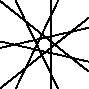
\includegraphics[height=1.5cm]{labsseptic1.pdf}
        &
        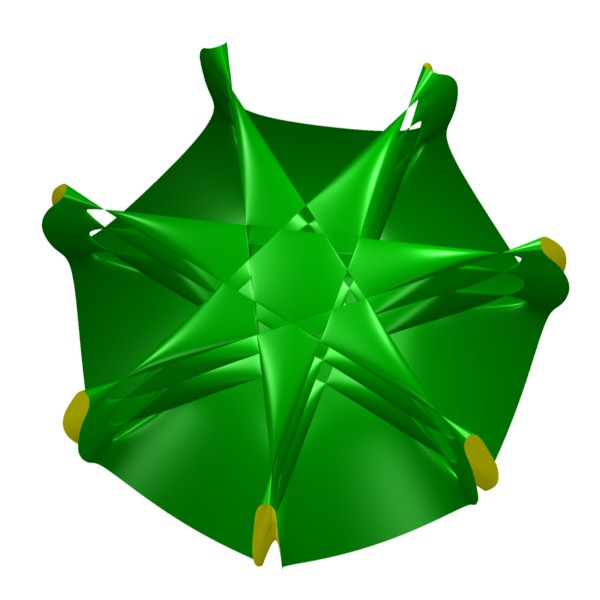
\includegraphics[height=1.5cm]{septic_7eck_von_oben}
      \end{tabular}
    \end{center}
    \vspace*{-0.3em}   
   Deze variant van Chmutovs constructie werd gemaakt door Duco van Straten.
\end{surferPage}
